\documentclass{article}
\usepackage{listings}
\usepackage{graphicx}
\usepackage{amsmath}
\usepackage[margin=3cm]{geometry}

\title{Operating manual: test data acquisition}
\begin{document}
\maketitle
 \section{Background}
 Firstly some background...
 \subsection{Load cell}
 A load cell is a device which can measure applied loads. Provided the applied load is sufficiently large, the output of the load cell $f_{cell}$ is a linear function of the applied load $F$, such that:
 \begin{equation}
  f_{cell}(F) = a\cdot F + b
 \end{equation}
 Where $a$ and $b$ are values to be obtained from calibration.

 \subsection{Time of flight sensor}
 The time of flight sensor measures distance by timing
 \subsection{I2C connections}
 Protocol for communicating between small devices (such as arduino's) using only 2 wires.

 \section{Setup}
 Interfacing with the data acquisition tool is done using Python. A few steps are required to set up the module. Firstly, you will require a functional installation of python 3. Then, install the PySerial module using pip in a command prompt:
 \begin{lstlisting}
  pip install pyserial
 \end{lstlisting}
 Start your python environment, and open the IAC\_data\_logging.py file. Run the script, and verify that you get output. Note that this is not real data, but instead data that is formatted in the same way for development purposes. The script will run perpetually, to halt it you can perform a keyboard interrupt using Ctrl+C. To acquire actual data, first power up and connect the device to your computer. The script will have provided some information about connected USB devices when you first ran it. If not, you can manually scan the USB ports by calling the port scan function in a python terminal:
 \begin{lstlisting}
  port_scan()
 \end{lstlisting}
 This will provide a list of all attached USB serial devices. Identify the relevant device in the list\footnote{Usually, this is formatted as ``COM\#'' with \# being a number} and note the USB port of the circuit. Fill in the USB port in the script options. Now, you can disable the development mode by setting:
 \begin{lstlisting}
  dev = False
 \end{lstlisting}
 Try running the script with development mode disabled, and verify that you obtain output.

 \section{Data processing}
 Several preparations have to be done in order to succesfully capture data during your experiment. While running, the program continuously acquires data through the USB connection. This data is structured as follows:
 \begin{lstlisting}
  load_cell VALUE time_of_flight VALUE
 \end{lstlisting}
 At each step, this data is stored in the \textit{line} variable. This data is stored as a \textit{string}. Your first task is to process this string in such a way that the data gets stored in a useful manner. Keep in mind that the script does not know when your experiment will end, and thus should be saving data continuously (not all at the end).\\

 Secondly, you should design a procedure for calibrating the sensors. The program will output pure numerical values, not actual measurements. This means you will have to tackle two problems:
 \begin{itemize}
  \item The sensors (particularly the load cell) might return a non-zero value when no input is applied. For example, when not loading the sensor, you might get a reading of $-5716$.
  \item The sensors do not return values in proper units. For example, when loading the sensor with 20 kilograms, you might obtain a reading of $28371$.
 \end{itemize}

\newpage

\section{Schematic}

\begin{figure}[htbp]
 \centering
 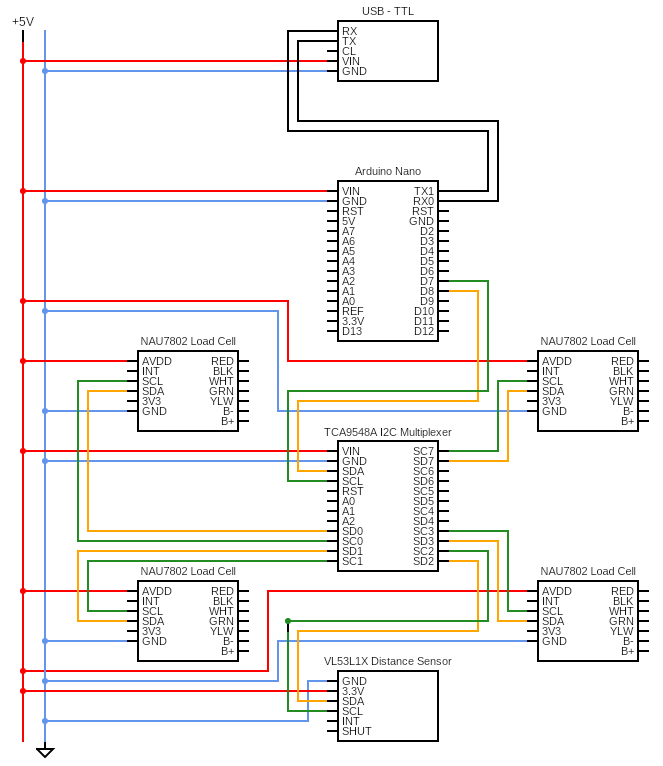
\includegraphics[width=0.9\textwidth]{circuit.png}
 \caption{diagram}
\end{figure}

\end{document}
